\documentclass[a4paper,12pt]{article}
\usepackage[a4paper, total={180mm, 272mm}]{geometry}

\usepackage{fontspec}
\setmainfont[Path=fonts/, Extension=.ttf]{ipaexm}

\setlength\parindent{3.5em}
\setlength\parskip{0em}
\renewcommand{\baselinestretch}{1.247}

\usepackage{graphicx}
\graphicspath{{images/}}

\begin{document}

\thispagestyle{empty}

\Large
\noindent \\
Spin Blur Ino\medskip
\par
\normalsize
Generate an average value Blur in the direction of rotation.\\
\par
First, it processes the Alpha channel, if specified.\par
Then, it handles the RGB pixels if the Alpha channel is not zero.\par
If you do not want to process to the Alpha channel, it will mask the changes in the\par
RGB image using the Alpha values. Therefore, smooth edges will remain smooth.\\
\\
-{-}- \ Inputs \ -{-}-\\
Source\par
Connect the image to process.\\
Reference\par
Connect the reference image to put the strength of the effect into each Pixel.\\
\\
-{-}- \ Settings \ -{-}-\\
Center\par
Specify the position of the center of rotation.\par
Origin is the center of the image to be processed. Not the gaze point of the camera.\par
The unit is millimeters.\par
The default value is the center of origin position at \textquotedbl 0.0 0.0\textquotedbl .\\
\\
Radius\par
Specify the range that does not get blurred from the center.\par
The unit is millimeters.\par
Enter a value greater than or equal to 0.\par
The default value is 0 which will be a total blur.\\
\\
Blur\par
The strength of the blur and adjustment.\par
The strength of the blur is specified in the rotation angle.\par
When the minimum value is 0 it does not do anything. The maximum value is 180.\par
The default value is 1.\\
\\
Type\par
Accelerator\par
\noindent \hskip 7em Blur angle,\par
\noindent \hskip 7em It can be strong enough to go to the outer periphery.\par
\noindent \hskip 7em The vertical height of the half position in the result image from the Center,\par
\noindent \hskip 7em specify the Blur angle, it will be weaker on the inside, and becomes\par
\noindent \hskip 7em stronger towards the outside.

\newpage

\thispagestyle{empty}

\ \vspace{-0.2em}
\par
Uniform\par
\noindent \hskip 7em  Whether it is close or far from the Center the Blur angle will be constant.\\
\par
The default setting is \textquotedbl Accelerator\textquotedbl .\\
\\
Alpha Rendering\par
When ON it will also process to the Alpha channel.\par
When OFF, it does not process to the Alpha channel,\par
It will mask the change of the RGB values using the Alpha values.\par
The default setting is ON.\\
\\
Anti Alias\par
Specify the process of adding antialiasing in order to eliminate any jaggies.\par
The result will become more smooth, but it will take more time to process the image.\par
The default setting is OFF.\par
<Processing time reference example>\par
Width=2176 Height=1236 Center=0,0 Radius=0 Blur=3 Alpha=ON\par
Shrink=1\par
\noindent \hskip 7em Type=Accelerator\par
\noindent \hskip 10.5em Anti Alias=OFF ~28sec\par
\noindent \hskip 10.5em Anti Alias=ON \, ~360sec\par
\noindent \hskip 7em Type=Uniform\par
\noindent \hskip 10.5em Anti Alias=OFF ~23sec\par
\noindent \hskip 10.5em Anti Alias=ON \, ~280sec\par
Shrink=3\par
\noindent \hskip 7em Type=Accelerator\par
\noindent \hskip 10.5em Anti Alias=OFF ~5sec\par
\noindent \hskip 10.5em Anti Alias=ON \, ~17sec\par
\noindent \hskip 7em Type=Uniform\par
\noindent \hskip 10.5em Anti Alias=OFF ~4sec\par
\noindent \hskip 10.5em Anti Alias=ON \, ~13sec\\
\\
Reference\par
Choose how Reference image values put the strength of the effect into each Pixel.\par
An image is connected to the \textquotedbl Reference\textquotedbl \ of the input,\par
Choose from Red/Green/Blue/Alpha/Luminance/Nothing.\par
Choose Nothing when you do not want this effect, it will turn off the connection.\par
The default setting is Red.

\newpage

\thispagestyle{empty}

\ \vspace{-0.2em}
\par
\noindent Spin Blur \ \ Reference Example

\large
\noindent \begin{picture}(0,0)
\put(170.5,-144.5){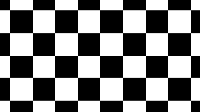
\includegraphics[width=13.3em]{SpinBlurInoOriginalImage}}
\put(92.5,-343){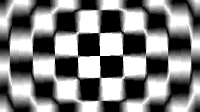
\includegraphics[width=13.3em]{SpinBlurInoUniformBlur11AAOFF}}
\put(314.5,-343){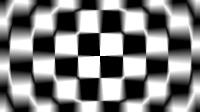
\includegraphics[width=13.3em]{SpinBlurInoUniformBlur11AAON}}
\put(92.5,-486){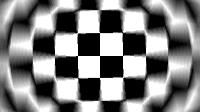
\includegraphics[width=13.3em]{SpinBlurInoAcceleratorBlur11AAOFF}}
\put(314.5,-486){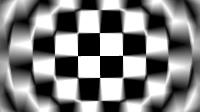
\includegraphics[width=13.3em]{SpinBlurInoAcceleratorBlur11AAON}}
\put(26,-50){\normalsize{Original Image}}
\put(26,-67){\normalsize{(200x112pixel)}}
\put(89,-221){\normalsize{Anti Alias \ \ OFF}}
\put(311,-221){\normalsize{Anti Alias \ \ ON}}
\put(26,-249){\normalsize{Uniform}}
\put(26,-267){\normalsize{(Blur\,11.25)}}
\put(26,-382){\normalsize{Accel-}}
\put(26,-400){\normalsize{erator}}
\put(26,-418){\normalsize{(Blur\,11.25)}}
\end{picture}\\[12.65em]

\end{document}